\section{Machine Learning in Mechanics}
%\begin{frame}{Side Track Brief History}
%\begin{minipage}{0.45\textwidth}
%  \begin{block}{\color{White} Second Boom\cite{Fradkov2020}}<1-2>
%    \begin{itemize}
%      \item <1> Civil \& Mechanical Engineering
%      \item <2> Functional approximations (mostly experimental data)
%    \end{itemize}
%  \end{block} 
%\end{minipage}%
%\hspace{1cm}
%\begin{minipage}{0.45\textwidth}
%  \begin{block}{\color{White} Gold Rush\cite{Fradkov2020}}<3-4>
%    \begin{itemize}
%      \item <3> Anything I can think of...
%      \item <4> My interest 
%    \end{itemize}
%  \end{block} 
%\end{minipage}
%\end{frame}

\begin{frame}{Constitutive Modeling}
\begin{center}
  $\nabla \cdot \boldsymbol{\sigma} =0 \to  $ Equilibrium Equation 
\end{center}
  
\begin{minipage}{0.45\textwidth}
  \begin{block}{\color{White} Computationally Material}<1-2>
    \begin{itemize}
      \item <1> Trying to learn $\boldsymbol{\sigma}=\mathcal{C}(\boldsymbol{\varepsilon})$ 
      \item <2> Any supervised learner
    \end{itemize}
  \end{block} 
\end{minipage}%
\hspace{1cm}
\begin{minipage}{0.45\textwidth}
  \centering
  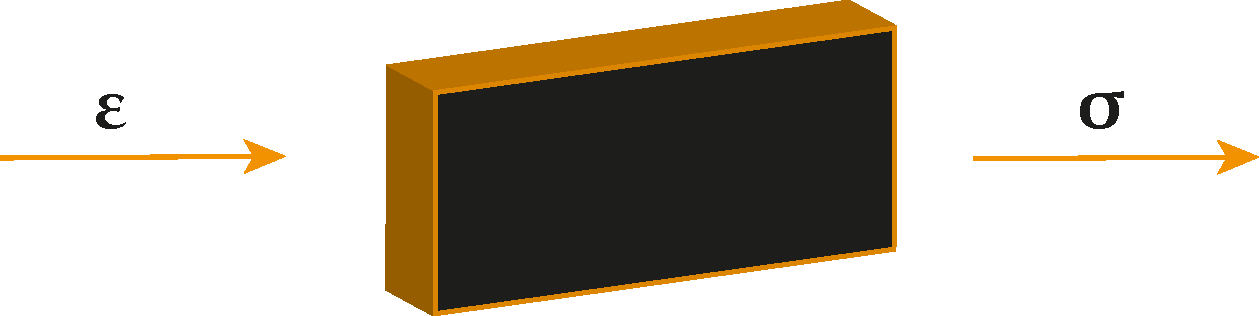
\includegraphics[width=0.8\textwidth]{Figures/surrogate/material.pdf}
\end{minipage}
\end{frame}

\begin{frame}{Constitutive Modeling}
\begin{center}
  $\nabla \cdot \boldsymbol{\sigma} =0 \to  $ Equilibrium Equation 
\end{center}
 
\begin{minipage}{0.45\textwidth}
  \begin{block}{\color{White} Assumptions}
   \begin{itemize}
      \item Geometry 
      \item Material Model
   \end{itemize}
  \end{block} 
  \only<2> {
  \centering
    $\Downarrow$
  \begin{block}{\color{White} Parametrizations Examples}
   \begin{itemize}
      \item $V_f$, $L$
      \item $E$, $\nu$
   \end{itemize}
  \end{block}}
\end{minipage}%
\hspace{1cm}
\begin{minipage}{0.45\textwidth}
  \centering
  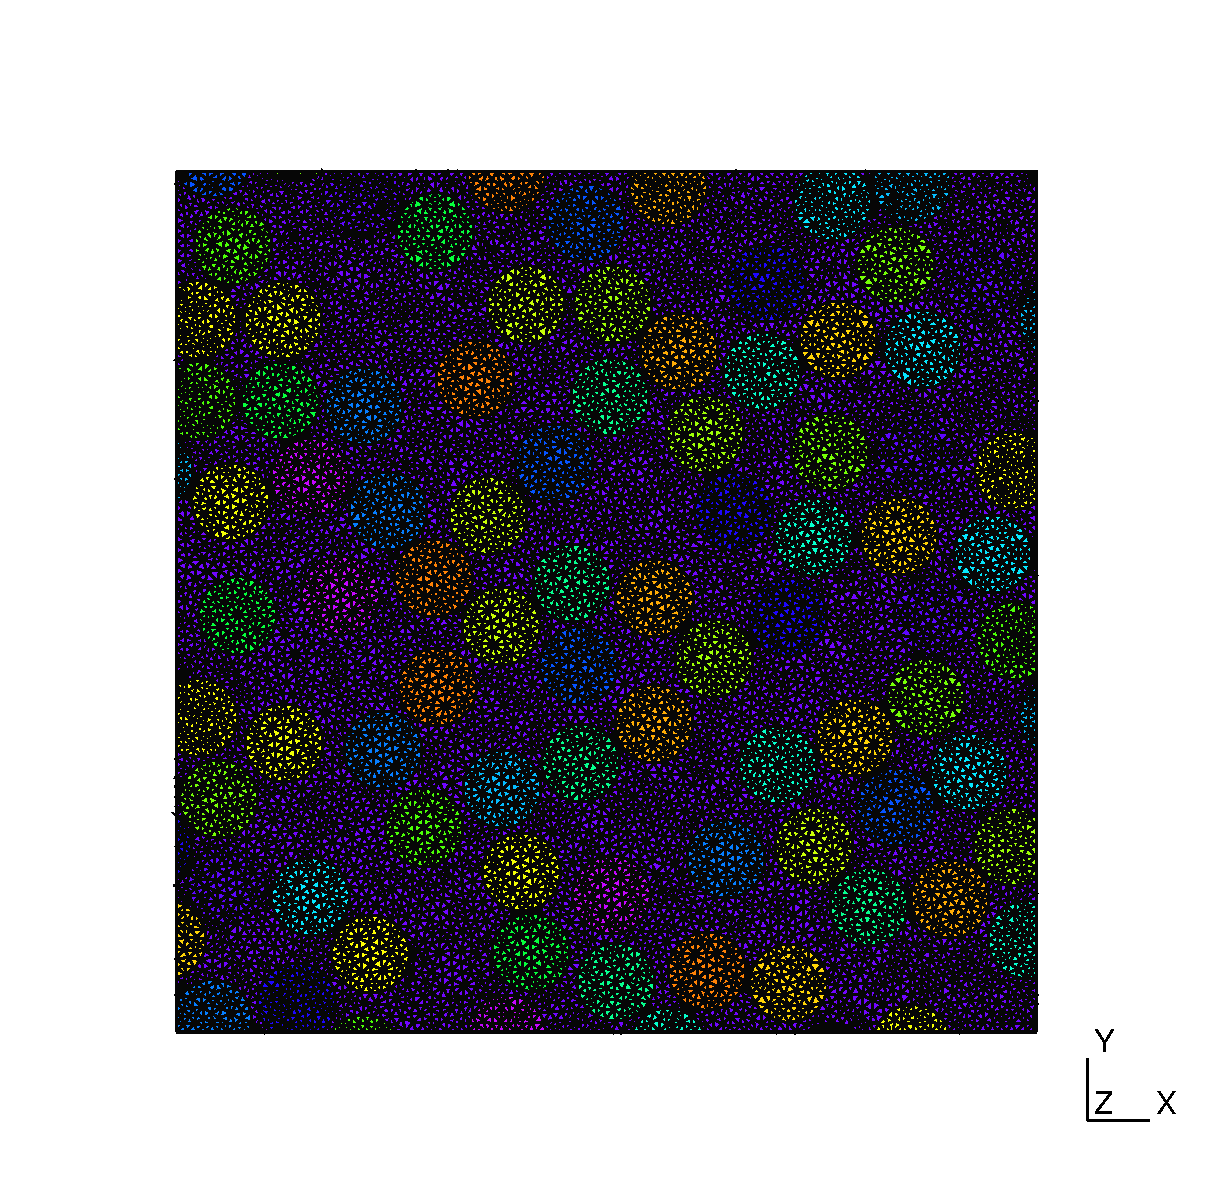
\includegraphics[width=0.9\textwidth]{Figures/surrogate/rve81.pdf}
\end{minipage}
\end{frame}

\begin{frame}{Current ML Approaches}
\centering
\begin{minipage}{0.8\textwidth}
    \begin{itemize}
      \item \textit{Physics-informed} ML models (SCA \cite{Liu2016b}, DMN \cite{Liu2019a}, etc.)
      \item Brute force fitting to parameters of interest \cite{Rocha2020},\cite{Bessa2017b}
      \item \textit{Physics-driven} ML models (PINN\cite{Raissi2017})
    \end{itemize}
\end{minipage}%
\end{frame}

